%%% Template for a snapshot of modern mathematics from Oberwolfach. Please use pdflatex for compiling this file.
\documentclass{snapshotmfo}

%%%%%%%%%%%%%%%% WILL BE FILLED OUT BY EDITORS ACCORDING TO YOUR SPECIFICATIONS ON IMAGINARY %%%%%%%%%%%%%
%\categorizationmath{algebra and number theory,analysis,discrete mathematics and foundations,geometry and topology,numerics and scientific computing,probability theory and statistics} %at least one must be chosen. 
%\categorizationconnect{chemistry and earth science,computer science,engineering and technology,finance,humanities and social sciences,life science,physics,reflections on mathematics} %can be void.
%\license{CC-BY-NC-SA-3.0} %recommended
%\license{CC-BY-NC-ND-3.0}
%\license{CC-BY-SA-3.0}
%\snapshotid{id}{year}
%\organizer{Main Organizer}
\junioreditor{will be filled out by editors}{junior-editors@mfo.de}
\senioreditor{Dr.\;Carla Cederbaum}{cederbaum@mfo.de}
\director{Prof.\;Dr.\;Gerhard Huisken}
%%%%%%%%%%%%%%%%%%%%%%%%%%%%%%%%%%%%%%%%%%%%%%%%%%%%%%%%%%%%%%%%%%%%%%%%%%%%%%%%%%%%%%%%%%%%%%%%%%%%%%%%%%


%%%%%%%%%%%%%%%% PLEASE FILL OUT THE FOLLOWING ITEMS %%%%%%%%%%%%%%%%%%%%%%%%%%%%%%%%%%%%%%%%%%%%%%%%%%%%%

%%% Optional recommended packages
%%% Encoding
\usepackage[utf8]{inputenc}
%%% AMS mathematical facilities:
\usepackage{amsmath,amssymb}
%%% Consistent quotation marks and citations:
%\usepackage{csquotes}
%%% Enhanced typesetting of units:
%\usepackage{siunitx}  
%\sisetup{per-mode=fraction,fraction-function=\nicefrac}

% Please feel free to use your own macros but please do not change the layout of the snapshot.

%%% Please select 'ngerman' if you want to submit your snapshot in German. If you do choose 'ngerman', please run your LaTeX compiler *twice* or delete the .aux file.
%\usepackage[ngerman]{babel}
\usepackage[USenglish]{babel}


%%% Please separate your names by \and if there are several authors.
\author{Author One \and Author Two}

%%% Please insert the title of your snapshot.
\title{Your title}

%%% Please provide some information on the author(s).
\authorinfo{\authorname{Author One} is professor for pure mathematics at the First University.\\\mailtoref{author.one@first.edu}}
\authorinfo{\authorname{Author Two} is lecturer for applied mathematics at the Second Institution.\\\mailtoref{author.two@uni-second.de}}


%%% Please provide your references here or as a .bib file. If you use a .bib file, please replace the bibliography name 'yourbibfile' with the name of your .bib file in the \bibliography command at the bottom of this file. If you prefer to use \bibitems, you will need to silence the \bibliography command at the end of this file (see below). 
\usepackage{filecontents}
\begin{filecontents}{\jobname.bib}
@book{knuth1986texbook,
  keywords = {book},
  title={The texbook},
  author={Knuth, D.E. and Bibby, D.},
  volume={1993},
  year={1986},
  publisher={Addison-Wesley}
}

@article{snapshot,
  title={The first snapshot},
  author={Jahns, S. and Renner, L.},
  journal={Snapshots of modern mathematics},
  volume={1},
  number={1},
  pages={1--10},
  year={2014},
  publisher={MFO}
}

@misc{ wikiMath,
   author = "Wikipedia",
   title = "Mathematics --- {W}ikipedia{,} The Free Encyclopedia",
   year = "2014",
   howpublished = "\url{https://en.wikipedia.org/wiki/Mathematics}",
   note = "[Online; accessed 19-May-2014]"
 }

@misc{sample13,
 author = {Sample, J.},
 howpublished = {arxiv:alg-geom/1306.3461v1},
 title = {Interesting facts in algebraic geometry},
 year = {2013},
}

@incollection{sample12,
 author = {Sample, J.},
 title = {Things you don't know about mathematics},
 booktitle = {A bookseries about mathematics},
 publisher = {Some publisher},
 year = {2012},
}
\end{filecontents}

%%%
%%%%%%%%%%%%%%%% If your latex file does not compile, please delete all .aux and .log files and try again. %%%%%%%%%%%%%%%%%%%%%%%%%%%%%%%%%%%%%%%%%%%%%%%%%%%%%
\begin{document}

%%% Please insert your abstract, here. 
\begin{abstract}
This is your abstract. It should give a brief overview of your snapshot. If possible, please do not use formulas in your abstract. Please do not use more than 300 symbols. You will be asked to copy your abstract into the upload form on \href{http://www.imaginary.org}{www.imaginary.org}. 
\end{abstract}

%%% Please insert the main body of your snapshot, here.
\section{A heading}
Your actual snapshot.\footnote{This is a footnote.} As usual, you can give references such as \cite{snapshot, knuth1986texbook, wikiMath, sample13, sample12} via the \verb+\cite+ command.\\

We appreciate if you include images or other graphics that illustrate your snapshot. However, please do keep in mind the copyright issues explained in our email in case you include images and graphics you have not produced yourself.

%%% Please use this format to include images. Supported image formats: jpg, pdf, png. Please convert your images to those formats.
\begin{figure}[h]
        \centering 
        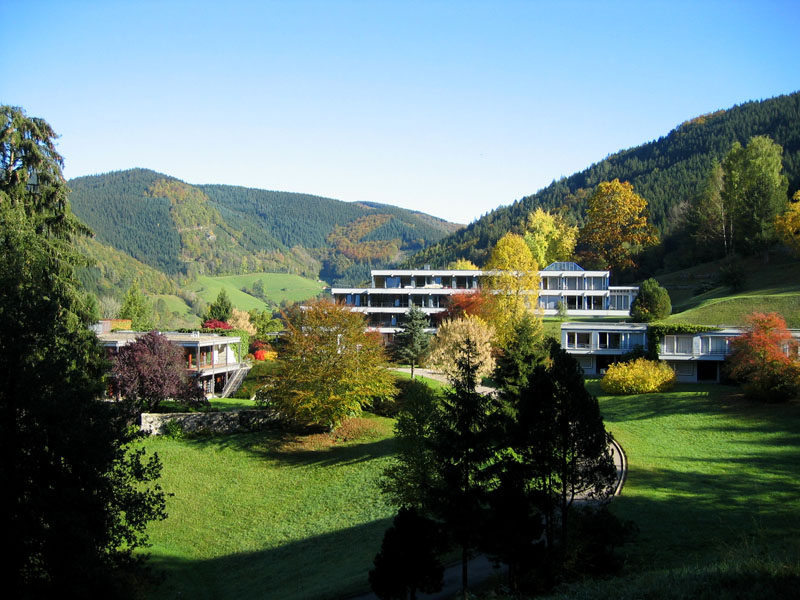
\includegraphics[width= 0.33 \textwidth]{sample-image.jpg}
        \caption{An image scaled to 33\% of the textwidth.}
\label{fig:sample-image}
\end{figure}

\subsection{A subsection}
More text and some formulas:
\begin{align}\label{real}
1+1&=2,\\\label{char.2}
1+1&=0.
\end{align}
Formula \eqref{real} refers to $\mathbb{R}$, formula \eqref{char.2} does not.

\section{More Information}
We have composed guidelines to help you write a beautiful and accessible snapshot which you can download here: \href{http://www.mfo.de/math-in-public/snapshots/guidelines-for-snapshots}{www.mfo.de/math-in-public/snapshots/ guidelines-for-snapshots}. For more information on the snapshot project (including example snapshots), please see \href{http://www.mfo.de/math-in-public/snapshots}{www.mfo.de/math-in-public/snapshots}.

%%%%%%%%%%%% Bibliography via BibTeX %%%%%%%%%%%%%%%%%%%%%%%%%%%%%%%%%%%%%%%%%%%%%%%%%%%%%%%%%%%%%%%%%%%%%%%%%%%%%%%%%%%%%%%%%%%%
%%% Please use this command in case you prefer to use the filecontents environment and edit your BibTeX entries above. If you prefer to use \bibitems, you will need to silence the \bibliography following command with a % symbol.
\bibliography{\jobname}

%%% Please use this command in case you supply your own .bib file. Replace 'yourbibfile' by the name of your .bib file. Please silence the above command \bibliography{\jobname} with a %-symbol. Also, please do not forget to *submit* your .bib file with your .tex file when uploading it on www.imaginary.org.
%\bibliography{yourbibfile}

\end{document}
